\documentclass[tikz,border=5pt]{standalone}
\usepackage{tikz}
\usetikzlibrary{arrows.meta}
\definecolor{nebula}{HTML}{6366F1}
\definecolor{spark}{HTML}{14B8A6}
\definecolor{ink}{HTML}{334155}
\begin{document}
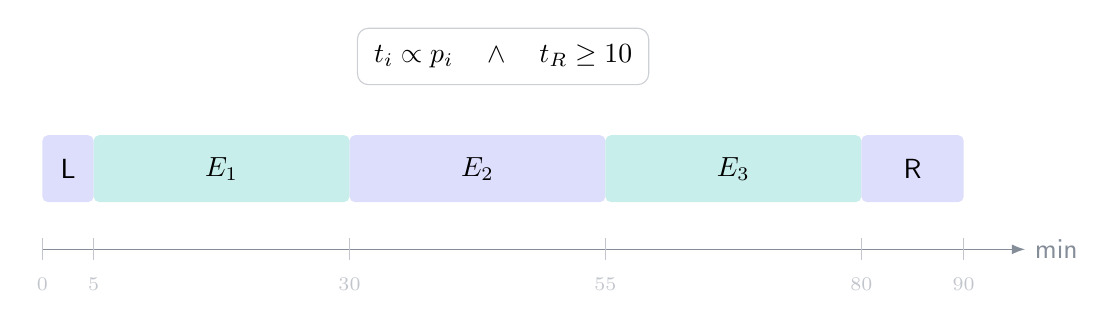
\begin{tikzpicture}[font=\sffamily,>=Latex,x=.13cm,y=1cm]
  \draw[->,ink!60] (0,0)--(96,0) node[right] {min};
  \foreach \x in {0,5,30,55,80,90}{\draw[ink!30] (\x,.14)--(\x,-.14) node[below=3pt,font=\scriptsize] {\x};}
  \fill[nebula!22,rounded corners=2pt] (0,.6) rectangle (5,1.45);
  \fill[spark!24,rounded corners=2pt] (5,.6) rectangle (30,1.45);
  \fill[nebula!22,rounded corners=2pt] (30,.6) rectangle (55,1.45);
  \fill[spark!24,rounded corners=2pt] (55,.6) rectangle (80,1.45);
  \fill[nebula!22,rounded corners=2pt] (80,.6) rectangle (90,1.45);
  \node at (2.5,1.02) {L}; \node at (17.5,1.02) {$E_1$}; \node at (42.5,1.02) {$E_2$};
  \node at (67.5,1.02) {$E_3$}; \node at (85,1.02) {R};
  \node[draw=ink!25,rounded corners=4pt,fill=white,inner sep=6pt] at (45,2.45)
    {$t_i\propto p_i\quad\land\quad t_R\ge 10$};
\end{tikzpicture}
\end{document}
